\chapter{Economics}\label{chapter:economics}

So far, we have analyzed our protocols in the \emph{honest majority} setting,
assuming that most parties will follow our protocol. We provided assurances
such as safety and liveness to honest parties. But it's not clear why,
even though these assurances are provided, anyone should follow our honest
protocol, especially if they can achieve better benefits by deviating from
it. If there is money to be made by violating the protocol, it is likely that
a majority of participants will do so. Instead of assuming \emph{honesty},
it would make more sense to assume that participants are \emph{rational}.
A rational party does not necessarily follow the prescribed honest protocol.
Instead, he may deviate from the rules in order to make money.
The ideal scenario would be if the honest protocol we designed is also
\emph{incentive-compatible}\index{Incentive Compatibility}:
that there is no better strategy that
a party can follow which deviates from the honest strategy and makes them
more money (a Nash equilibrium).

\section{Rationality Models}

There are a few different models in which we can analyze our protocols.
In the \emph{cryptographic} model, the majority of parties are assumed
to be honest (and PPT), whereas the rest are allowed to be arbitrarily
adversarial (they can be any PPT algorithm). In the \emph{game theoretic}
model, \emph{all} parties are typically assumed to be rational, and
no computational restrictions are imposed upon them. However, the game
theoretic model does not typically account for adversaries who are willing
to deviate from the protocol even if they are about to lose money. Such
parties can be realistic in cases where, for example, a nation-state
wishes to invest resources simply to shut down a decentralized protocol.
But the cryptographic model \emph{does} capture such adversaries, as
long as most other participants are honest.

It would be nice to capture the best of both worlds. The most powerful
results would be achieved in a model where a \emph{majority} of parties
are assumed to be PPT rational, whereas a minority are assumed to be
\emph{arbitrarily PPT adversarial}. This is holy grail model and its
comparison to the other models is depicted in Figure~\ref{fig.rationality}.
Unfortunately, analyzing protocols in the rational majority setting
is very difficult with the current mathematical tooling available to us.
Analyzing the incentives of blockchain protocols is only possible for
very simple protocols, or for very simple models, and having an arbitrary
PPT adversary in the picture makes things even harder. While we would
like to have analyses in this model, it is rarely the case that we can.
There are many reasons for this, among others the complexity of the protocol,
the large number of parties, the broad range of available strategies,
the fact that the protocol is iterated over large periods of time,
and the fact that the practical instances of these protocols have externalities
such as payments that can be received outside of the protocol.

\begin{figure}[h]
  \centering
  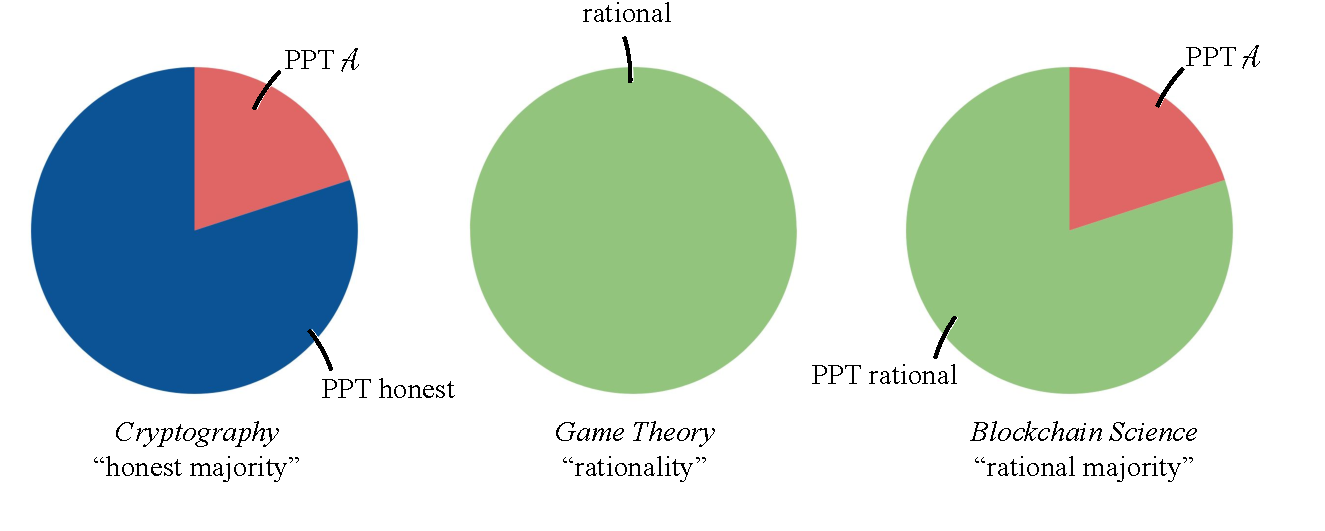
\includegraphics[width=\columnwidth,keepaspectratio]{figures/rational-model.pdf}
  \caption{The cryptographic, game theoretic, and blockchain science model.}
  \label{fig.rationality}
\end{figure}

Regardless of the limitations of our understanding and ability to prove
things precisely in the rational majority setting, it is still worthy
to think about the rationality of our design. While we might not be able
to prove that our honest protocol is incentive-compatible and survives against
arbitrary adversaries, we also want to make sure the honest protocol is
not costly to operate without providing appropriate incentives to honest
participants.

In the particular case of the proof-of-work protocol we have studied,
running the honest mining protocol is actually extremely costly. At the time of
writing, Bitcoin consumes more electricity than the whole country of Argentina,
which is an expensive endeavour. Therefore, miners need to be incentived to
secure the network, for example by having their electricity paid for.

We have already examined the mechanisms by which miners are paid when they
successfully mine a block in Chapter~\ref{chapter:chain}, where we mandated
that a block's coinbase transaction pays out a total amount $f_t$ which
consists of the \emph{block reward} $f_r$ and the \emph{block fees} $f_f$:

\[
    f_t = f_r + f_f
\]

Both of these terms are denominated in the system's native currency. We
will now study these two terms in more depth.

\section{The Block Reward}
The block reward part constitutes the \emph{macroeconomic policy} of the
system. This block reward plays a dual role for the system: Firstly, it
incentivizes miners to participate in the honest protocol. Secondly, it
is a natural mechanism for the decentralized creation of money. Whereas
the first purpose is necessary to make the protocol incentive-compatible,
the second part is a policy decision of the protocol. For example, it is
equally possible to have protocols in which new money creation is left up
to a central party, which can be the party to whom the newly issued money
is paid out to, and only a small proportion of the proceeds to go to the
miner. This would centralize money issuance, but still enable decentralized
public verifiability. Such decisions are a matter of policy.

The exact algorithm determining the value of $f_r$ is \emph{hard-coded}
into each full node and is part of the block validation algorithm. When
a block is validated, its coinbase is also validated, and this is where
the macroeconomic policy is checked for validity. It is typically not
possible to change these rules of the cryptocurrency, unless the community
of the currency all decide to move to a new policy and upgrade their software
together. Such decisions can be difficult and contentious.

% TODO: Write a small section on hard/soft forks and blockchain upgrades in
% this chapter.

There are a few alternatives that can be followed in the macroeconomic
policy of a cryptocurrency. The policy is defined as a function of the
block $f_r(B)$. One option is to make the reward \emph{constant}, which
means that the total supply will continue increasing at a constant rate.
Another option is to make the reward \emph{decreasing} over time until
it becomes $0$. In such a system, the function $f_r$ depends on the block
height. With such a policy, the total supply is increasing over time, but
converging to a particular value.

This is the policy that Bitcoin follows.
Bitcoin's macroeconomic policy is an interesting concrete example, because
many other cryptocurrencies follow a similar policy. The function $f_r$
for Bitcoin follows a staircase pattern, with long periods of constant
supply per block. The supply began at a rate of $50$ bitcoin per block
at genesis. Every four years in block time (which corresponds to
$210{,}000$ blocks because $\eta = 10$ minutes in Bitcoin), the reward
per block drops to a half (a process known as \emph{reward halving}).
The reward schedule for Bitcoin therefore
began at $50$ bitcoins per block during the years 2008-2012, dropped
to $25$ bitcoins per block during the next four years, and so on. At
some point in the future the block reward in Bitcoin will drop below
one Satoshi, at which point it will become $0$ and no new coins will
enter the supply. In about a century, Bitcoin will reach a total supply
of $21$ million bitcoin, and the reward will drop to $0$. This
macroeconomic policy is depicted in Figure~\ref{fig:reward_halving}
(in this graph by CoinDesk, \emph{subsidy} refers to the block
reward).

\begin{figure}[ht]
    \centering
    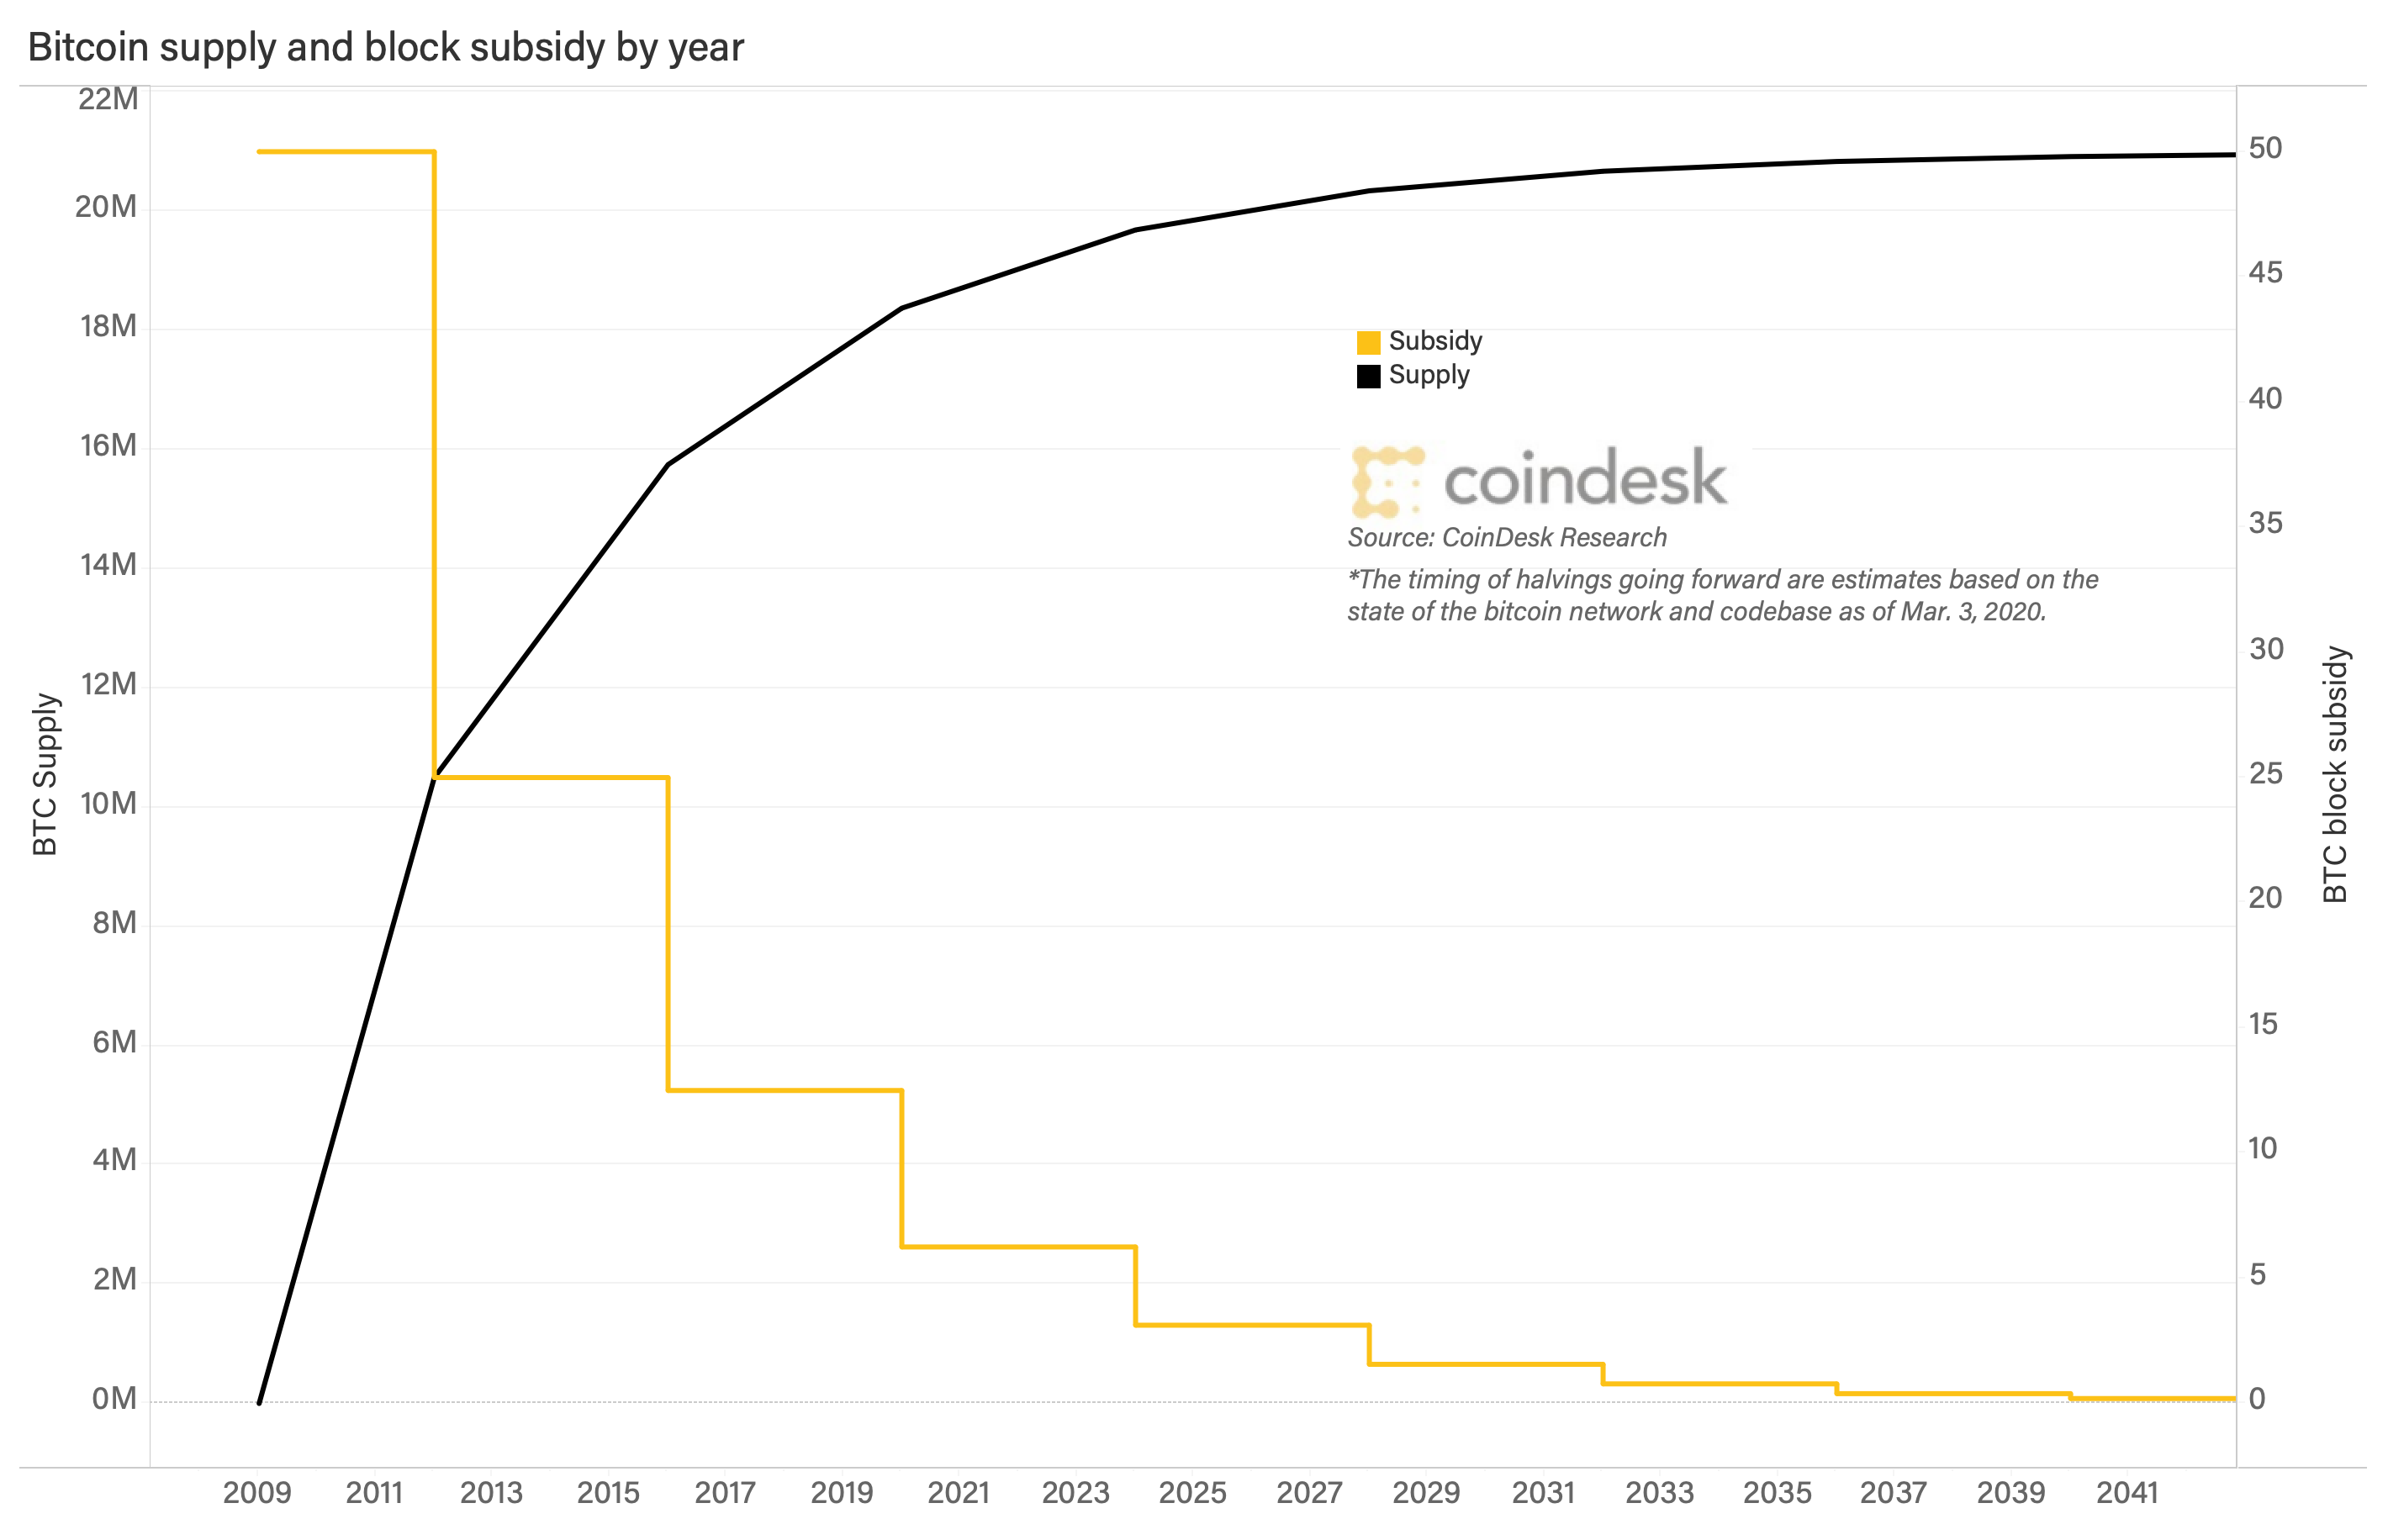
\includegraphics[width=\columnwidth,keepaspectratio]{figures/reward_halving.png}
    \caption{Reward Halving for Bitcoin Supply (source: coindesk)}
    \label{fig:reward_halving}
\end{figure}

One of the problems with such a policy is that the reward function
$f_r(h)$ is discontinuous with block height, and the finite difference
of the total supply function $\sum f_r$ changes abruptly at the points of
reward halving. This behavior can cause market shocks because the incentives
to the miners shift abruptly. Consider a miner who has invested in a large
business to mine blocks. The cost of electricity to mine is a certain
amount. At the moment of reward halving, the miner is still spending
the same amount per month in electricity, but only getting half of the
nominal rewards. Electricity is typically paid out in fiat (i.e., non-crypto)
currency such as USD. If the price of Bitcoin in USD remains the same, then
the miner will be forced to stop half of their operation overnight.
Alternatively, if the miner is to continue operating at the same rate,
the price of Bitcoin in USD needs to double overnight. Both of these
are undesirable situations.

To avoid such market shocks, other cryptocurrencies have adopted a more
nuanced macroeconomic policy. One such example is Monero which pioneered
the concept of \emph{smooth emission}. In such a system, the rewards
are reduced slightly in every block, following a pattern similar to
Bitcoin's macroeconomic policy, but adjusted to work in a more continuous
manner.

The reward and total supply functions for Bitcoin and Monero are
illustrated in Figure~\ref{fig.macroeconomics}. The actual
reward and supply over real (and not block) time can fluctuate less smoothly
than anticipated because of the stochastic nature of proof-of-work.
Note how Bitcoin's block reward forms a staircase, while Monero's
is a smooth curve. Due to a decision taken by the community, Monero's rewards
flatten out at the point indicated by the vertical red line.

% TODO: redo this figure
% https://www.reddit.com/r/Monero/comments/512kwh/useful_for_learning_about_monero_coin_emission/
\begin{figure}[h]
  \centering
  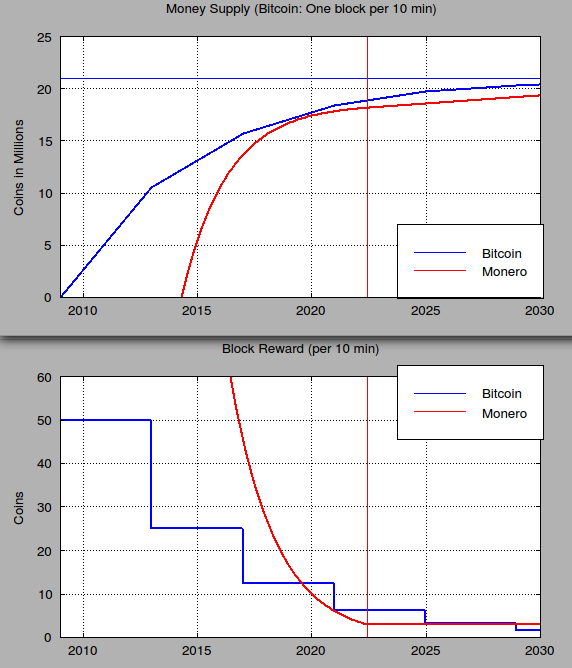
\includegraphics[width=0.8 \columnwidth,keepaspectratio]{figures/macroeconomics.png}
  \caption{The total supply (top) and block reward (bottom) for Bitcoin and Monero.}
  \label{fig.macroeconomics}
\end{figure}

Because the total supply stops growing at some point in time, Bitcoin
and Monero are \emph{deflationary cryptocurrencies}. Many orthodox
economists believe that deflationary cryptocurrencies are inappropriate
as currencies, because they encourage hoarding and not spending when
the emission period is over. This is one reason why other cryptocurrencies
have no limit on their total supply. Instead, they continue to inflate
the currency and are therefore known as \emph{inflationary cryptocurrencies}.
While it is important that the total supply of a cryptocurrency is limited
at every point in time to ensure scarcity, it is not necessary that there
is a global total bound across all of time. One such example cryptocurrency
is Dogecoin.

Overall, the decision of the macroeconomic policy of a system is up to
the economists and the community, and there is no exact science that can
define it in an objectively acceptable manner. Any emission algorithm
which is socially acceptable by the economic participants can be used.

The block reward is the main way miners are incentivized to mine.

\section{Miner Fee Optimizations}

While miners are incentivized to mine blocks by giving them a block reward,
they need to also be incentivized to include transactions in their blocks.
Otherwise, they will simply create \emph{empty blocks}\index{Empty Block},
blocks that contain only a coinbase transaction and don't confirm any
part of the mempool. This is solved by introducing transaction fees.

The other term of the total payout is the fees $f_f(B)$ of a block $B$.
Recall that the fees are calculated as the excess money that goes into
a transaction but does not go out. Given a transaction $\tx$ in the UTXO
model, the fees that this transaction is paying will be

\[
   \sum_{i \in \tx\textsf{.ins}} i.v - \sum_{o \in \tx\textsf{.outs}} o.v\,.
\]

The creator of a transaction can choose how many fees he wants to pay,
and these can be $0$ or larger.

Each block contains many transactions, each of which may pay out fees. All
these transaction fees make up the \emph{fee} part $f_f(B)$ of the block payout:

\[
  f_f(B) = \sum_{\substack{\tx \in B.\overline{x}\\\tx \textsf{ non-coinbase}}}
           \left(\sum_{i \in \tx\textsf{.ins}} i.v - \sum_{o \in \tx\textsf{.outs}} o.v\right)\,.
\]

Including an extra transaction has minimal cost to the miner and does not affect the mining
rate. If there was no limit in how big blocks can be, a rational miner would include all
transactions paying even minimal fees. But contrary to what we have described so far,
we will need to introduce a block size limit so that our assumptions can work out.

\subsection*{The Block Size Limit}

So far, we have not imposed any limits on how big blocks can be. We have also assumed
that blocks can traverse the network within $\Delta$ time, just like any other network message.
This should make you a bit suspicious by now. The larger a block is, the more time it
takes to send over the network. If we don't impose a bound on how large a block can get,
then $\Delta$ cannot be a fixed constant. There are some simple ideas to make blocks of
bounded size that don't work. One such example is to include just the transaction ids
within the block, and then allow the client to request each transaction as needed at
a later time. Another example is to just include the hash of the transaction sequence
$\overline{x}$, which already commits to the transactions, and not the transactions
themselves, again allowing the interested client to download the transactions in question.
We'll explore these strategies in more detail in Chapter~\ref{chapter:light} to optimize
our protocol, but for now let's observe why these don't fix the $\Delta$ problem:
The time $\Delta$ really captures the time that is needed for \emph{all} the data
to transmit over the network so that a block can be properly validated. If we separate
out transaction bodies from blocks, then a miner who observes a new block on the network
has to download all transactions in order to ensure block validity. Otherwise, the
miner cannot know if the block is valid or not and where to mine.

\glsxtrnewsymbol[description={block size limit}]{block size limit}{$\Bmax$}\glsadd{block size limit}
To ensure our assumption of a $\Delta$ delay holds, we will limit the size of a block
to $\Bmax$:

\[
    |B| \leq \Bmax
\]

This size limit must be denominated in actual \emph{bytes} (or bits) transmitted
over the network, not in the number of transactions per block. The reason is that the delay
$\Delta$ depends on the literal size of the object transmitted.

% TODO: Talk about how $\Delta$ can be decreased and the nodes who don't receive messages
% can be counted as part of the adversary, but this reduces the resilience. Maybe in a different
% chapter.

\subsection*{Miner Strategies}

Generally speaking, which transactions to include in a block is completely up to the miner,
as long as the block ends up being valid. The miner can choose to leave the block empty,
fill it to the brim, include transactions that are paying small fees, or include transactions
paying large fees. The miner can also include their own transactions at any position they
want within the block, and reorder the rest of the transactions in the block in any way
they like. Despite all of this freedom, some transaction inclusion \emph{strategies} are better than
others.

A rational miner is looking to optimize the fees that they can gain by including the highest
paying transactions that they can. When the miner is mining, they create a template block
in which the included transactions are $\overline{x}^*$. This $\overline{x}^*$ is computed
as follows. If the transactions in their mempool $\overline{x}$, plus
the new coinbase transaction, are enough to fit within $\Bmax$, then the miner has no reason
to exclude any transactions. He can simply include everything to maximize his profits.

On the other hand, if the mempool $\overline{x}$, plus the new coinbase transaction, exceed
the block size limit $\Bmax$ in size, then the miner must make a choice on which transactions
to include. He tries to maximize the profits by including the highest paying transactions.
In order to do that, each transaction is associated with a \emph{score}\index{Transaction Score}.
The score of a transaction is defined as the fees it is paying divided by the bytes it takes up:

\glsxtrnewsymbol[description={transaction score}]{transaction score}{$\score$}\glsadd{transaction score}
\[
    \score(\tx) = \frac{|\tx|}{\sum_{i \in \tx\textsf{.ins}} i.v - \sum_{o \in \tx\textsf{.outs}} o.v}
\]

The easiest way is then to order transactions by score, in descending order, and take
transactions until no more fit and $\Bmax$ would be exceeded. This strategy is also known
as the \emph{greedy strategy}\index{Greedy Strategy}. The reason why the ratio fee/byte
is used instead of just the fee is that, naturally, a bigger transaction takes up more space in
the block, and must therefore pay accordingly. This concept that block space costs a certain
amount per byte is also known as \emph{block space rent}\index{Block Space Rent}.

% TODO: write the greedy strategy in pseudocode

Unfortunately for the miner, things are not so simple. The first issue that arises is that
transactions can either be included \emph{as a whole} or \emph{not at all}. It is not possible
to cut a transaction in half and just include a portion of it into the block. This means that
the strategy to just include the top-score transactions will not perform optimally. One
such example is illustrated in Figure~\ref{fig.rational-miner-txs}. Here, the block is
illustrated as the outer blue box, with its size indicating the block size limit $\Bmax$.
Transactions in the mempool (breaking away from our usual circle
notation) are displayed as smaller boxes containing numbers. The numbers within the transactions
indicate their score, and the size of a box indicates the transaction's size in bytes.
The transactions have been ordered by the greedy strategy from left to right in
descending order according to their scores. The green transactions are included in
the block, as they are the transactions with the top scores. The red transactions
are not included in the block, as they have lower scores. The transaction with
a score of $4$ barely doesn't fit in the block. However, the greedy strategy misses
the fact that the two smaller transactions with a score of $3$ can both still fit in
the block. A more clever solution would include these also. If it were possible to cut the
transaction with the score of $4$ and partially include it, then this solution would
have been optimal, but we are forced to exclude it altogether, so the transactions
with a score of $3$ are our next best option.

\begin{figure}[h]
  \centering
  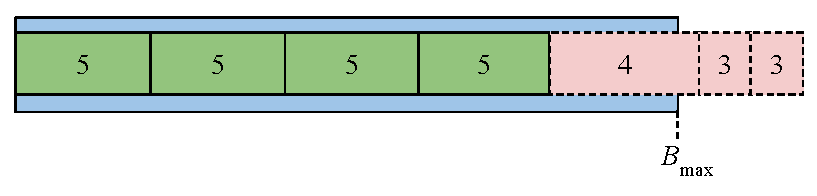
\includegraphics[width=0.8 \columnwidth,keepaspectratio]{figures/rational-miner-txs.pdf}
  \caption{The greedy strategy is not always optimal.}
  \label{fig.rational-miner-txs}
\end{figure}

This problem is known as the $0/1$ Knapsack problem and is known to be an NP-hard problem.
Its best known solution is only pseudopolynomial (which means it takes exponential time to
execute). Therefore, the problem of optimizing
which transactions to include is, generally, difficult, and only heuristics can be employed
to solve it. These heuristics sometimes necessarily yield suboptimal solutions.

Even this simple rendition of the problem is NP-hard, but in fact the problem is harder still.
The transactions that can be included must also respect the topological order induced by
the transaction graph. We cannot include a transaction $\tx_1$ before the transaction $\tx_2$
it is spending from. Therefore, the problem is similar to a $0/1$ Knapsack, except that
topological relations must also be preserved.

Lastly, there is one more complication. The simplistic honest miner maintains a mempool
that outright rejects double spends. This is fine for a miner who is not interested in
maximizing his profits. However, a rational miner wants to keep track of double spends.
If two conflicting transactions $\tx$ and $\tx'$ are available, the miner wishes to
choose the one with the highest paying fee. Even if a double spending transaction does
not pay large fees, it may still worth be caching for later inspection, because it may
be the input to a next transaction that \emph{does} pay large fees. Therefore, a rational
miner will also cache transactions outside of his mempool and hold onto them in case
they are later helpful in optimizing his profits.

In complex blockchains, such as Ethereum, the order of transactions in a block may give rise
to more nuanced profits than just those obtained from fees, and so even more advanced techniques
are needed. The strategies employed by modern rational miners to optimize profits are extremely
complicated and have given rise to a whole industry on their own. In the modern world,
\emph{computing} the near-optimal $\overline{x}^*$ and actually \emph{mining} a block
are two separate tasks. The computation of $\overline{x}^*$ is a task performed by
\emph{searchers} and \emph{builders}, whereas the mining is performed by \emph{miners}.
These are different, somewhat mutually trusted, parties running different software and
communicating with one another to optimize rational block production and share these
profits, which can range to tens of millions of dollars per month.

\section{Wallet Fee Optimization}

While the miner is trying to \emph{maximize} their fees, the \emph{wallet} of the user
who is spending money is trying to \emph{minimize} their fees. What is observed on-chain
is the economic equilibrium between the two.

Refer back to Figure~\ref{fig.wallet-fullnode-architecture} to recall that the wallet
is the piece of software that sits between the human user and the full node. The job of
the wallet is to take requests from the human user to make payments, and to issue the relevant
transactions to make these payments. The human user places such a request by choosing a particular
recipient and value to transfer. It is up to the wallet to decide how to build the transaction.

The timeline is roughly as follows. First, the human user places a request to the wallet
to make a payment of amount $v$ to some recipient $pk$. The wallet receives the human
request. The wallet then decides an amount of fees per byte (the score) that it wishes to spend
on the transaction to be created. Based on this score and an estimation of the size of the
transaction which will be created, it estimates the total fee $\phi$ that the transaction is about
to pay out. It then builds a new transaction
$\tx$, with an output of value $v$ and recipient $pk$. It then asks the full node for
the current UTXO set. Among the UTXO set, the wallet (which maintains a set of private keys)
can distinguish those outputs that belong to the user, since they correspond to addresses
encoding public keys that it holds the respective private key to. It then can make a choice
of outputs. This choice must make up a value of at least $v + \phi$, but can also exceed $v + \phi$.
The wallet adds those outpoints as inputs to the transaction. If the total value in the input
exceeds $v + \phi$, then it also adds a change output whose value is the total value of the
inputs reduced by $v + \phi$. The address in the change output is the encoding of a public
key of a new private key it generates and stores internally for future spending. After
the choice of inputs has been completed, the wallet inspects the new transaction for
its size and may adjust the $\phi$ amount accordingly. Overall, this is a heuristic
process.

Some aspects of the above procedure are worth explaining in more detail. The step of choosing
the inputs of the transaction must be done so as to minimize the total transaction size.
The size of each outpoint is roughly the same, so what needs to be minimized is the number
of inputs. Additionally, if the change output can be avoided, this is also desirable to
reduce the size of the transaction. So, one strategy is to simply consume all the largest
outputs that the user owns until the value $v + \phi$ is reached. However, this is not
necessarily the best strategy, as this may lead to future transactions that are more expensive.
Generally, there is no exact answer to this problem, because the wallet cannot know what
future values the user will want to spend. An ideal wallet would minimize the user's fees
across all of his spending habits. Different wallets employ different heuristics to reduce
the cost.

One more detail of the above procedure is to determine the score that the wallet wishes
to use for the upcoming transaction. To estimate the score, the wallet asks the human
user roughly how soon he wants the transaction to become confirmed by being included in
a block. This choice is a tradeoff between confirmation latency and cost in fees.
If the user wishes for fast confirmation, then the fees must be high.
If the user is willing to wait for some time, then the fees can be low.
If the fee is too low, the transaction may take a long time to be included,
or may even never be included.
The user sets a desired confirmation time $u$ (in, say, minutes).
The wallet knows that blocks are produced in expectation every $\eta = \frac{1}{f}$.
Once the transaction makes it to a block, it will take another $k$ blocks for it
to become confirmed (recall that $k$ is the confirmation parameter).
As such, the wallet attempts to adjust the score so that the
transaction makes it within the next $\frac{u}{\eta} - k = uf - k$ blocks.
The wallet then inspects the most recent $(uf - k)$ chunk of the currently
adopted blockchain by the full node $\chain[{-(uf - k)}{:}]$, sorts transactions
by score, and takes the minimum score. If the next $(uf - k)$-long chain chunk
about to be mined happens to behave similarly to the last $(uf - k)$-long chunk, then using this score
will ensure that the transaction will (marginally) make it within the next
$uf - k$ blocks, and so will become confirmed within $u$ time.

Some improvements
in this heuristic can be made by looking into older chunks and taking an average
to ensure that recent blocks are not outliers. Also, instead of simply taking the
minimum score, the wallet can consider several among the minimum-scoring transactions,
considering that the miners of recent blocks may have injected some transactions
of their own with a very low score. Of course, the mining process is stochastic,
and so blocks may not appear exactly $\eta$ apart. Additionally, the network
may become more congested, and people will tend to increase their fees in
that case. Fee estimators are inherently inaccurate. They can only function
heuristically and hope for the best.

If the fee of a transaction is miscalculated and it takes too long to make it
into a block, there is a strategy to rectify this. The user can issue a new
double spending transaction that spends from all the exact same outputs, but
pays a higher fee by including a smaller amount in its \emph{change} output.
This new transaction can then be broadcast to the network. Because miners are
rational, they will choose to adopt this transaction instead of the lower-fee-paying
alternative which already exists in their mempool. Such transactions are often
issued by wallets in practice and are known as \emph{replace by fee}\index{Replace by Fee}
transactions, and do not constitute attacks.
They are double spends, but are not inherently malicious.
While we previously said that only the adversary issues double spend,
now that fees have been introduced, it also makes sense for honest wallets
to do so on occasion. An example \emph{replace by fee} transaction is illustrated in
Figure~\ref{fig.replace-by-fee}.

\begin{figure}[h]
  \centering
  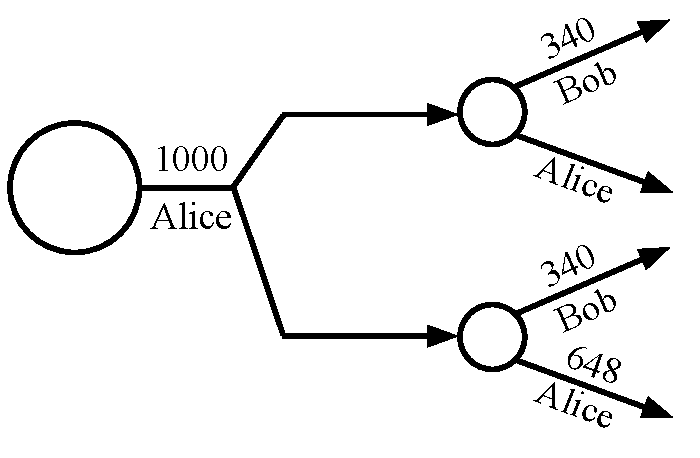
\includegraphics[width=0.4 \columnwidth,keepaspectratio]{figures/replace-by-fee.pdf}
  \caption{A replace-by-fee transaction. The same transaction is recreated, but with
           a lower value on the \emph{change} address.}
  \label{fig.replace-by-fee}
\end{figure}

\section{Types of Wallets}

The most risky part of a wallet concerns the responsibility of maintaining the
secret key private. A \emph{software wallet} that runs on a mobile phone or a
laptop computer stores the secret keys encrypted with a user-provided password
at rest. These are safe for storing small amounts of money.

For larger amounts,
a dedicated device known as a \emph{hardware wallet}\index{Hardware Wallet}
is used. These wallets are USB devices that can be connected to a computer
using a USB cable. They are responsible for generating a $(sk, pk)$ key pair
by invoking the signature scheme's $\Gen$ function. The secret key $sk$ never
leaves the hardware wallet, and this is enforced at the hardware level. The
wallet sends the $pk$ to the computer so that the computer can generate the
address to receive money. The computer also has the responsibility
of building transactions based on human user requests. These unsigned
transactions are then sent to the hardware wallet to obtain a signature.
Before signing the transaction, the hardware wallet will prompt the human
user for confirmation on the hardware device, displaying the total amount
to be paid and the recipient address. When the transaction is signed by
the hardware wallet and sent to the computer, the computer can then
broadcast this transaction to the network.

The hardware wallet ensures that, in case the computer becomes compromised,
the adversary cannot exfiltrate the secret key. Even if the adversary
places a request for a signature to the hardware wallet, the human user
will see the request and reject it. The hardware wallet is also protected
by a PIN that must be entered by the user before any transactions can be
signed. Rate limiting mechanisms for repeated PIN trials are enforced at
the hardware level. The hardware is built in such a way that, even when physical
access to the wallet is gained by the adversary, it is somewhat difficult
to extract the private key or generate a signature, although the protection
mechanisms at the hardware level have historically been subject to various
attacks, which were later patched.

Two popular hardware wallets in the current market are Ledger and Trezor.
Their photographs appear in Figures~\ref{fig.ledger} and~\ref{fig.trezor}.

\begin{figure}[h]
  \centering
  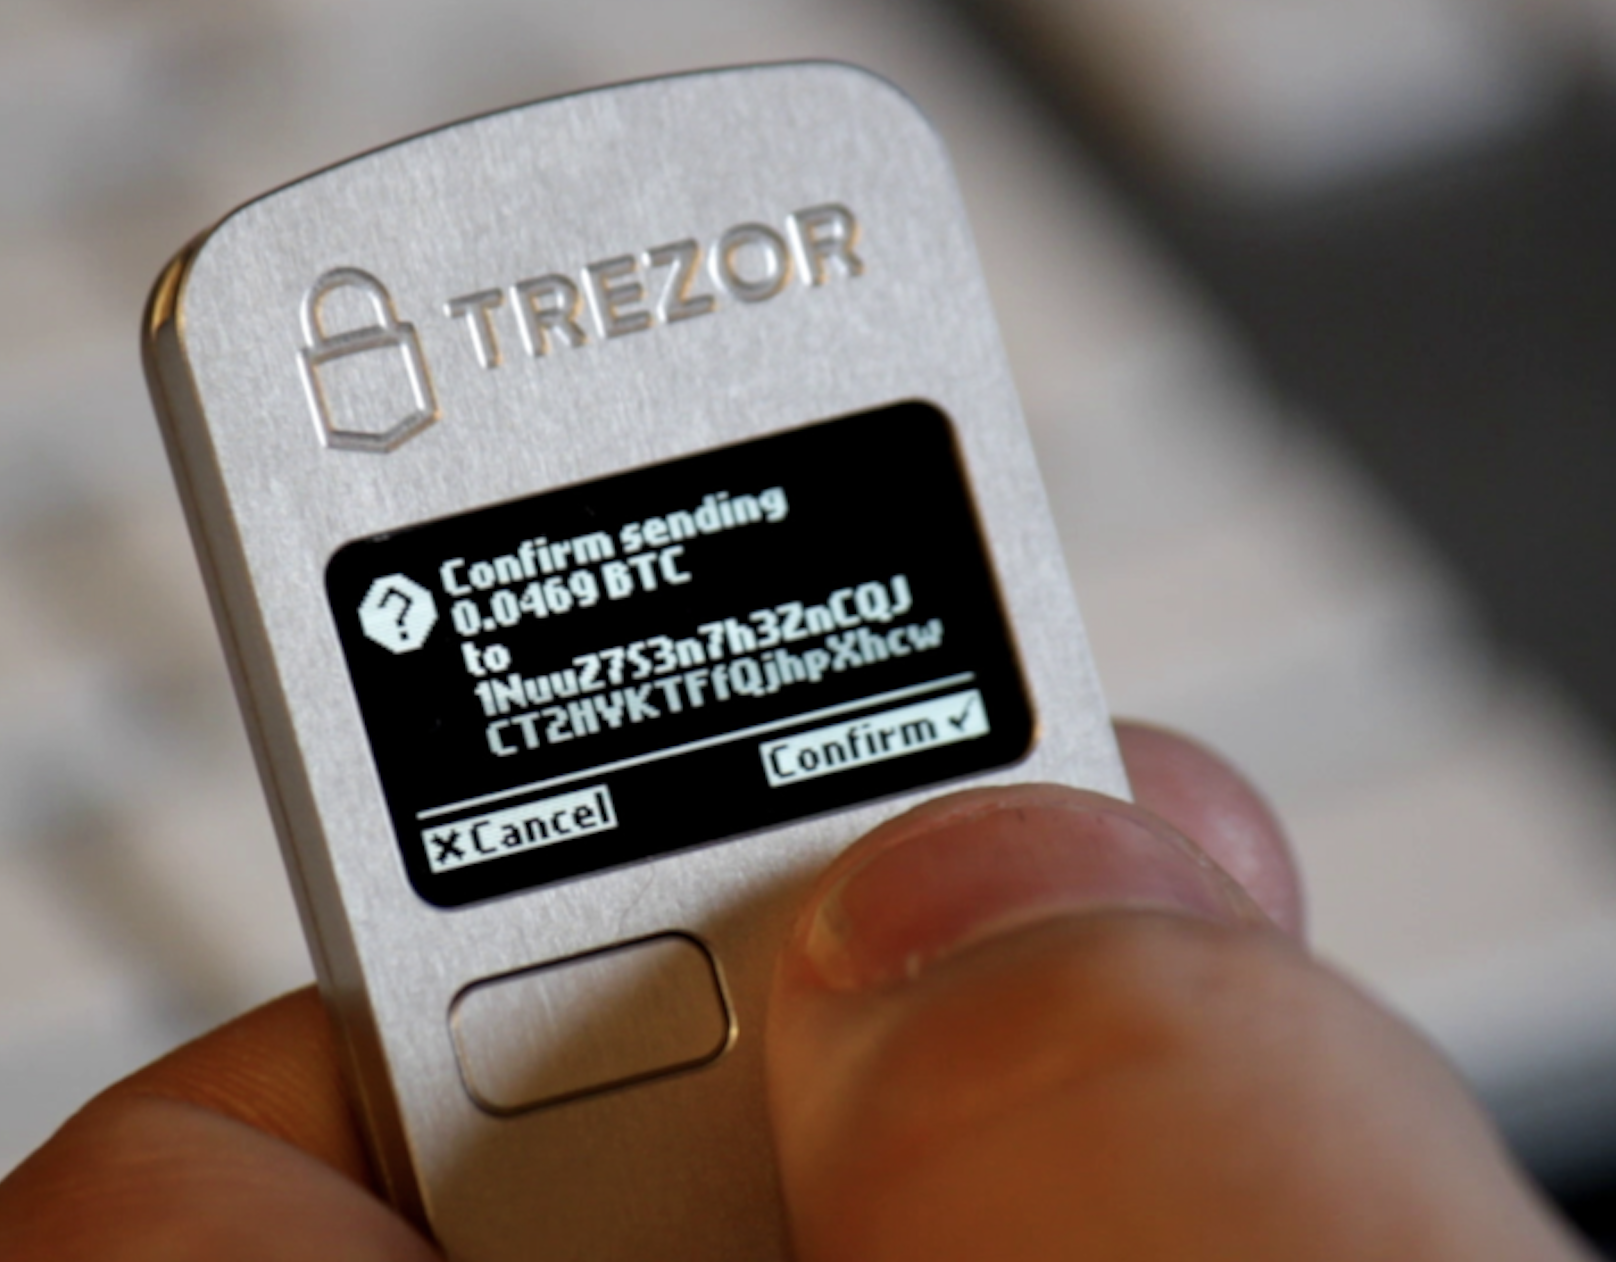
\includegraphics[width=0.7 \columnwidth,keepaspectratio]{figures/trezor-tx.png}
  \caption{A Trezor hardware wallet requesting human confirmation for a transfer.}
  \label{fig.trezor}
\end{figure}

\begin{figure}[h]
  \centering
  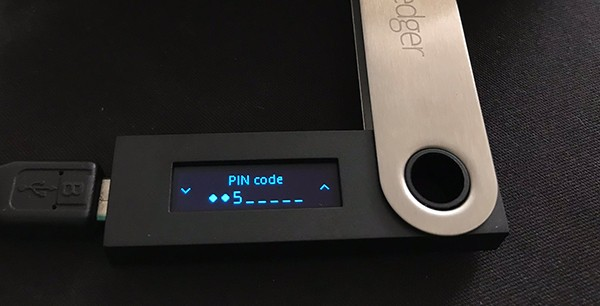
\includegraphics[width=0.7 \columnwidth,keepaspectratio]{figures/ledger-pin.png}
  \caption{A Ledger hardware wallet connected to a computer using a USB cable and
           requesting human input of the PIN.}
  \label{fig.ledger}
\end{figure}

We have already discussed that multiple secret keys can be generated so that
some basic level of pseudonymity is achieved by the wallet. Many wallets in the
UTXO model generate a new public/secret key pair every time they receive a new
payment. In contrast, in the accounts model, an account (which corresponds to
a public/secret key pair) is typically generated only when the user requests
so. Regardless of the model, wallets can be asked to generate and store
a series of secret keys. If this generation happens anew every time a key
is requested, this can be problematic, because the human user may have
kept a backup of the keys at an earlier time, and the backup will have to
be taken again. Instead of generating a brand new key every time it is
needed, wallets often make use of a \emph{seed}\index{Seed}. The idea
of a seed is that it is a master secret key on which all other secret
keys are based.

The seed is generated by sampling a $\kappa$-bit randomness uniformly at
random. This randomness is then encoded into a list of human-readable
dictionary words by splitting up the seed into chunks and using the chunk
as an index within a predetermined word list. Through this mechanism,
the human-readable version of the seed can be encoded to something that
looks as follows:

\begin{quote}
\texttt{online response lounge afraid}
\texttt{slow renew bright ritual}
\texttt{boring cram taxi page}
\end{quote}

Different cryptocurrencies use a different number of words and different
word lists, so these seeds may look different. Some cryptocurrencies include
checksums in their encodings so that some errors of transcription can be
detected.

The secret keys can then be generated from the initial seed. One simple way to do
this is to take the seed and hash it together with a counter $i = 0, 1, 2, \cdots$
to obtain the respective secret key. The first secret key is $H(\mathrm{seed} \conc 0)$,
the second secret key is $H(\mathrm{seed} \conc 1)$ and so on.
This method requires that the signature scheme has a mechanism of deriving
the public key from the secret key, and that its $\Gen$ function returns a
secret key uniformly at random from $\{0, 1\}^\kappa$, except with negligible
probability. Some signature schemes that are used in cryptocurrencies (for example
many elliptic curves) follow this form more or less, with some care required to
translate the hash output into the appropriate format for the private key.

In practice, a slightly more complex mechanism is used to derive the secret keys from
the seed, which allows generating keys for multiple different cryptocurrencies from
one shared seed. Such constructions are known as \emph{hierarchical deterministic wallets}
(HD-wallets)\index{Hierarchical Deterministic Wallet}. The details of such constructions
pertain to the engineering of the various cryptocurrencies.

% TODO: brain wallets

\section{Variable Difficulty}

As we briefly discussed in the healing section of Chapter~\ref{chapter:attacks},
it is possible for the adversarial power $t$ to fluctuate, and for the system to
alternate between periods of honest majority and dishonest majority.
Honest mining power $n - t$ can also fluctuate. In our calculations for the target $T$,
we have assumed that all the system parameters, including $n$ and $t$ remain
constant. In reality, however, mining power wildly fluctuates. As a blockchain
system becomes more popular and the price of its token increases,
more rational mines join the system hoping to make profit from it. This functions
as a reinforcement mechanism for its security: The more value a system stores,
the more miners tend to want to mine for it because it is more profitable, and
the more expensive it becomes to attack, because the adversary needs to
expend a lot of money to reach a high $t$ value. However, it is also possible
at times for the system to be undersubscribed by miners.
At the same time, as technology improves, the $q$ value also tends to increase with time.
It is not rare for popular systems to see a tremendous increase of mining
power over time. As an example, Bitcoin's hash rate in the unit of time ($nq$
in our terms, assuming the adversary is also mining in her full capacity)
is illustrated in Figure~\ref{fig.bitcoin-hashrate}. This
hash rate is not directly observable, but can be deduced by the block
production rate and the proof-of-work target $T$.

% TODO: redo this figure in perfect LaTeX vector format/pdf
\begin{figure}[h]
  \centering
  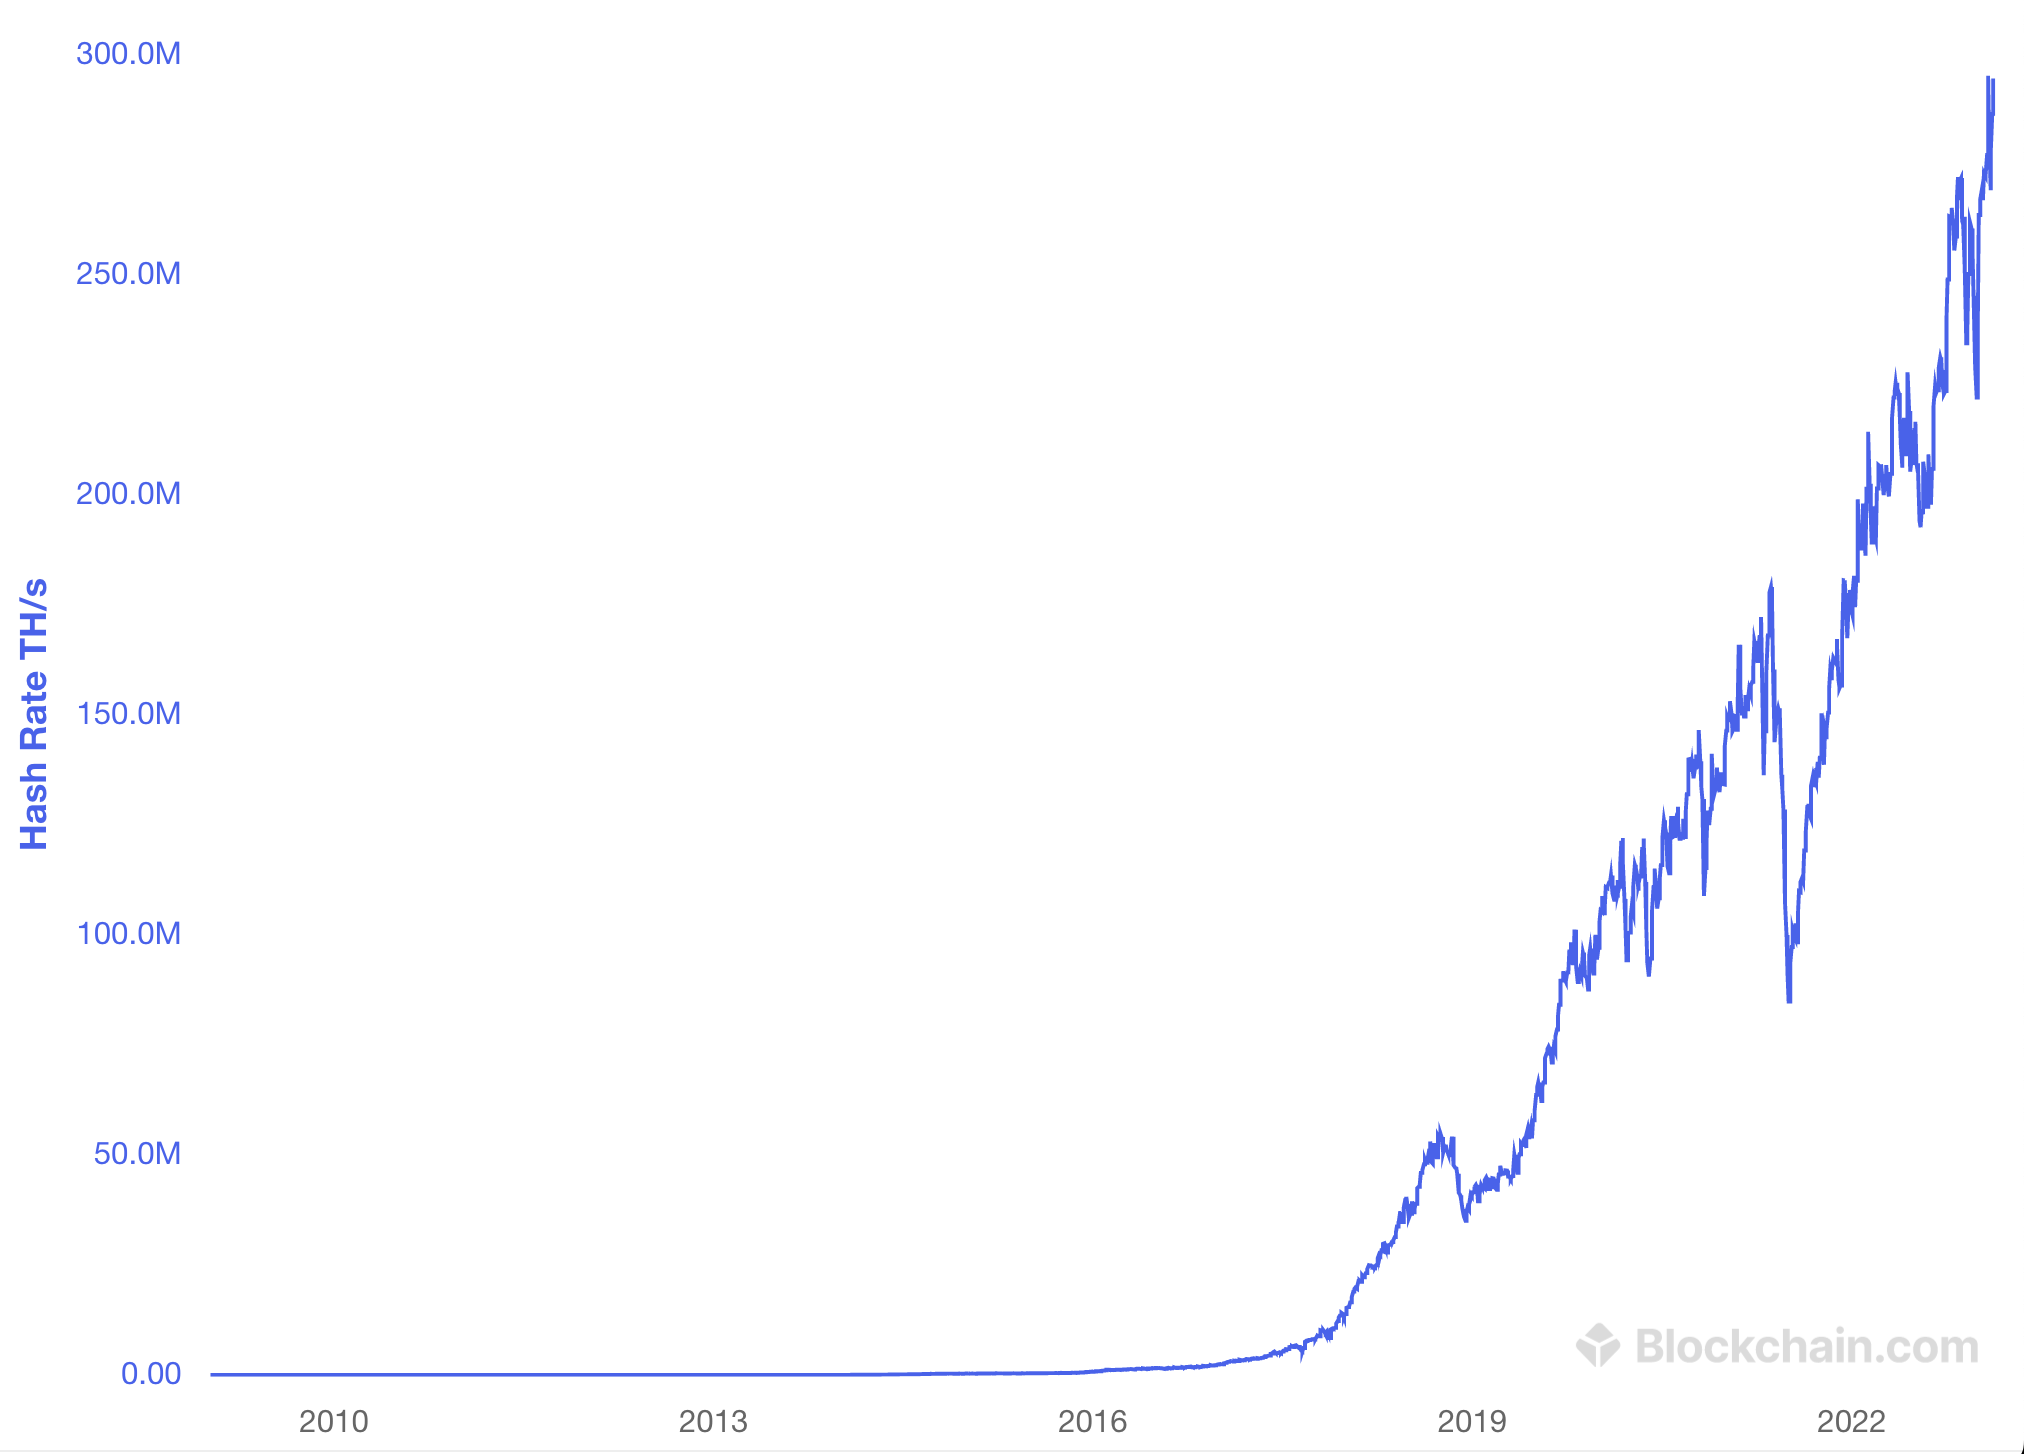
\includegraphics[width=\columnwidth,keepaspectratio]{figures/bitcoin-hashrate.png}
  \caption{Bitcoin's hash rate from its inception to 2023.}
  \label{fig.bitcoin-hashrate}
\end{figure}

When we calculated the $T$ parameter, we based our calculations on $n$ and $q$.
As these values change over time, the parameter $T$ will need to be adjusted.
Otherwise, successful queries may become too rare or too dense, leading
to issues of liveness or safety respectively.

When the system was first launched, the $T$ parameter was calibrated
according to the network parameter $\Delta$, which we assume does not
change much over time (a change in $\Delta$ implies technical innovations
on the physical network level, which we do not treat in this book),
% TODO: discuss using a hard fork to upgrade $\Delta$?
and the mining power $nq$ which existed at the first stages of the
system's lifetime. Based on the estimated $\Delta$, the system
was calibrated in order to achieve a particular expected block
generation rate $\eta$. For example, in Bitcoin, the system was
calibrated to achieve an $\eta$ of 10 minutes per block.
We wish this $\eta$ to remain constant throughout the system's
execution, even though the mining rate may fluctuate wildly.
We cannot directly measure the values $n$, $t$, and $q$,
but we can sample $\eta$ by taking observations now and
then, and making adjustments to $T$ accordingly. If $\eta$
is too large, this means that blocks are arriving farther
apart than we like, so we must increase $T$ to make mining
easier. If $\eta$ is too small, this means that blocks
are arriving close together, so we must decrease $T$ to make
mining harder.

As mining is a stochastic process, it can happen that a block
here and there may arrive quickly or slowly simply by chance,
not having to do with the actual underlying mining rate. Therefore,
we will not recalibrate our system every time a block arrives.
Instead, we'll choose a somewhat large number of blocks
and recalibrate the system every this many blocks. We call this
number of blocks $m$, the \emph{epoch duration}. Every $m$
blocks, the target $T$ is recalculated based on how quickly
these $m$ blocks arrived. The target $T$ remains the same
for the next $m$ blocks. These $m$-long chunks of blocks
in which the target remains the same are known as \emph{epochs}.
These epochs are illustrated in Figure~\ref{fig.pow-epochs}.

\glsxtrnewsymbol[description={epoch duration}]{epoch duration}{$m$}\glsadd{epoch duration}
\index{Epoch}
\begin{definition}[Epoch]
  Given an \emph{epoch duration} $m \in \mathbb{N}$,
  an \emph{epoch} of a chain is any chunk $\chain[im{:}(i + 1)m]$
  for any $i \in \mathbb{N}$.
\end{definition}

It is desired that each epoch takes $\eta m$ time to complete.
By measuring how much time it \emph{actually} took to complete,
we can proportionally adjust the target $T$. However, we cannot
do this by simply measuring \emph{when} we locally received a block,
because different nodes may disagree about the time at which
they received the block. Instead, we use the chain itself to
reach consensus about when a block was produced. We augment
our block structure by adding one more field to it: The time $r$
at which it was generated. Our block format now looks like
this: $B = s \conc \overline{x} \conc \ctr \conc r$.

% TODO: redo all figures in tikz
\begin{figure}[h]
  \centering
  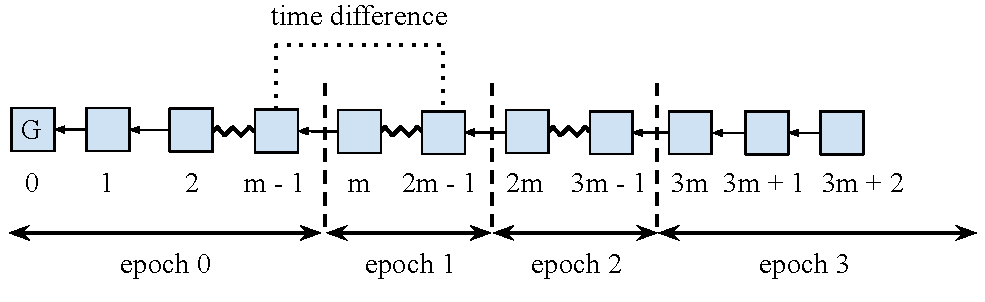
\includegraphics[width=0.8 \columnwidth,keepaspectratio]{figures/pow-epochs.pdf}
  \caption{Epochs of $m$ blocks in which difficulty remains fixed. Squiggly lines
           illustrate that some blocks have been omitted from the figure.}
  \label{fig.pow-epochs}
\end{figure}

Given this new block format, we can now adjust our difficulty at
the first block of every epoch, namely when a block's height is
divisible by $m$. For each $i$ with $i \equiv 0 (mod m)$ marking
the beginning of the epoch, we look at $\chain[i].r$, the timestamp
reported at the beginning of the next epoch, and compare it against
the timestamp $\chain[i - m].r$, the timestamp at the beginning
of the previous epoch. The difference $\chain[i].r - \chain[i - m].r$
marks the \emph{actual} time the epoch reportedly took. This must
be compared to the value $\eta m$, the \emph{expected} time
the epoch \emph{should}
have taken. Calculating the ratio between the two gives us the
target for the $j^\text{th}$ epoch:

\index{Target Recalculation}
\index{Difficulty Adjustment}
\[
    T_j = T_{j - 1} \frac{\chain[jm].r - \chain[(j - 1)m].r}{\eta m}
\]

This process is known as \emph{difficulty adjustment} or \emph{target
recalculation}. If the actual time is larger than the expected time,
the difficulty is decreased. If the actual time is smaller than the
expected time, the difficulty is increased.

Lastly, we need to ensure that the $r$ written on a block is somewhat
accurate. We do this by ensuring that the chain is \emph{temporally consistent},
which involves performing the following checks. Given a chain $\chain$:

\begin{enumerate}
  \item For all $i$, check that $\chain[i].r \leq \chain[i + 1].r$, i.e. timestamps are non-decreasing.
  \item Check that $\chain[-1].r$ is not in the future by comparing it to the local clock.
\end{enumerate}

The last check may cause a block to be rejected if the receiving party
has a clock that is slightly off. This is fine, because the party will
receive the block again later from others as it is rebroadcast through
the network. These two checks are added to the chain validation procedure.

These two simply checks make the timestamps reported on the chain quite
accurate. A minor adversary cannot lie about timestamps significantly.
Due to the unfavorable conditions of the Nakamoto race against the minor
adversary, the adversary cannot mine on top of a very old block. The
adversary can only mine on top of a recent block. Specifically, it only
makes sense for the adversary to mine on top of a block in
$\chain[{-k}{:}]$, because any attempt to mine on top of older blocks
will be in vain if $k$ Common Prefix holds. This means that the adversary
has a very small wiggle room about fraudulently reporting timestamps:
She can only place her timestamp between $\chain[{-k}].r$ and the current
timestamp. This means that the adversary can have a small adverse effect
on the difficulty recalculation, but this is not particularly significant.
These small timing variations are not very important, because such errors
can already happen in the system as it is. One reason for this is the
stochastic nature of proof-of-work.
The second reason is that the minor adversary can already cause the mining rate to fluctuate
by close to a factor of $2$ by simply turning her mining power on and off.
Therefore, small timing variations in difficulty recalculation are not very important.
It's the big picture that counts. This means that the value $\eta$ should be
calculated to be large enough so that, even under these small fluctuations
(which can range to more than a factor of $2$) should not affect safety.

At this point, it should be clear that $\eta$ must be chosen to be significantly
larger than $\Delta$ to achieve a good density of convergence opportunities.
We will calculate good values for $\eta$ (or, equivalently, its inverse $f = \frac{1}{\eta}$)
precisely in the next few chapters.

% TODO: bring these back
% \section{Some Bitcoin Statistics}
% We can take a look at the blockchain statistics for Bitcoin on the website:\\
% \href{https://www.blockchain.com/charts/hash-rate}{https://www.blockchain.com/charts/hash-rate}.
% Today, the hash rate of the bitcoin network is $210.48$m TH/s, measured in terahertz per second, as shown in Figure ~\ref{fig:hash_rate}. This can be denoted as:
% \begin{align*}
%     q\cdot (n-t) \approx 2^{67} \texttt{ Hz}.
% \end{align*}
%
%
%
% We can estimate the value of $q$ (the hash power of 1 party) on a real computer. On a laptop, $q \approx 100 \texttt{MHz}$. On a GPU, we can raise this to $q \approx 20 \texttt{ GHz}$. Today, we also use specialized mining power, with the best machines (ASICs) achieving $q \approx 200 \texttt{ THz}$. To see the hash power of the ASIC machine, you can refer to this website: \href{www.asicminervalue.com}{www.asicmine
% rvalue.com}
%
% We can also use the website to examine the number of transactions that are confirmed in any time frame. Here are some other observations:
% \begin{itemize}
%     \item The number of transaction spikes in the weekdays and toughs on the weekends
%     \item The number of UTXOs grew significantly in the past year
%     \item The mempool size is more erratic
% \end{itemize}
% Overall, observe that many network activity values depend on human factors.

% TODO: bring these back
% \begin{definition}
%     Let $f$ be the probability of getting an honest block in one unit of time. Then,
% \begin{align*}
%     f &\approx p \cdot q \cdot (n-t) \\
%     f &= 1- (1-p)^{q(n-t)}
% \end{align*}
% where $(1-p)^{q(n-t)}$ is the probability that every honest party failed.
% \end{definition}
% In Bitcoin, where 1 block is produced approximately every 10 minutes, we have $f \approx 1/600$ seconds. For small $p$, we have
% \begin{align*}
%     (1-p)^{q(n-t)} \approx 1 - qp(n-t)
% \end{align*}
%
% \begin{definition}
% Let $\eta = \frac{1}{f}$ be the expected block production duration.
% \end{definition}
%
% \section{Mining Pools}
% The probability of an individual miner successfully mining a block (and earning \$200k for the reward) is low. This reward has a high expectation, but it also has high variance. However, the miners want a consistent return, with the same expectation but a lower variance. To do this, miners combine together to form a \textit{pool}.
%
% \begin{definition}
% A \textit{pool} is a collaboration of miners. If any one miner succeeds, then they share the profit with other miners.
% \end{definition}
%
% \subsection{How Pools Work}
% The pool operator, a trusted party, generates a key pair ($pk, sk$) and shares the public key $pk$ with all miners. The participants mine the block, in which the coinbase transaction goes to the public key $pk$ of the pool operator. Then, the operator distributes profits to the miners.
%
% Now the pool operator must verify that the miners are actually mining. They could achieve this by setting up a light PoW verification.
% \begin{definition}
% The \textit{light PoW} equation provides a target that is significantly easier, called a \textit{light block share}:
% \begin{align*}
% H(B) &\leq 2^\xi T
% \end{align*}
% where $\xi$ denotes a constant that scales the target.
% \end{definition}
% The participants would send the light PoW block to the operator once they have mined a block. The operator validates that:
% \begin{enumerate}
%     \item The light block share satisfied the light PoW equation
%     \item The coinbase pays the operator\end{enumerate}
%
% Finally, after the block is mined, the operator distributes profits in proportion to the shares reported. An adversarial miner can only get payed if they submit the valid light block share. Additionally, the miner cannot change a valid block's public key to their own address because this will change the hash. Finally, an adversary would want to share a found block because they would get rewarded as part of the pool.

% \section{Wallets}
%
% \subsubsection{Types of Wallets}
% Wallets can be ``hot" or ``cold". Hot wallets are online, so they are easily available to use but less secure. Cold wallets are stored offline, such as in a hardware wallet or written down on a piece of paper. The hardware wallet could be plugged into a computer. The computer would store the transaction information, while the wallet generates the public keys, secret keys, and the signature without the secret keys leaving the device. They are more secure but tend to be harder to operate.
%
%
% \begin{figure}[ht]
%     \centering
%     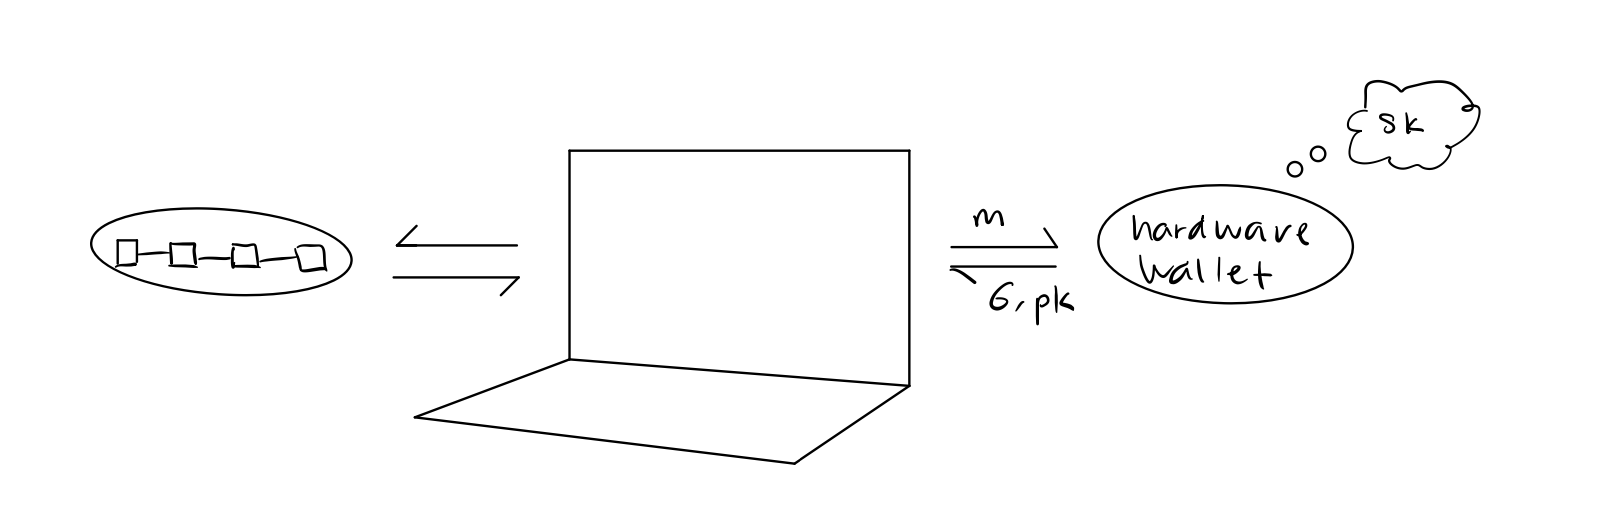
\includegraphics[scale = 0.5]{figures/hardware.png}
%     \caption{Illustration of the interactions between the hardware wallet and the computer}
%     \label{fig:hardware}
% \end{figure}
%
% \begin{figure}[ht]
%     \centering
%     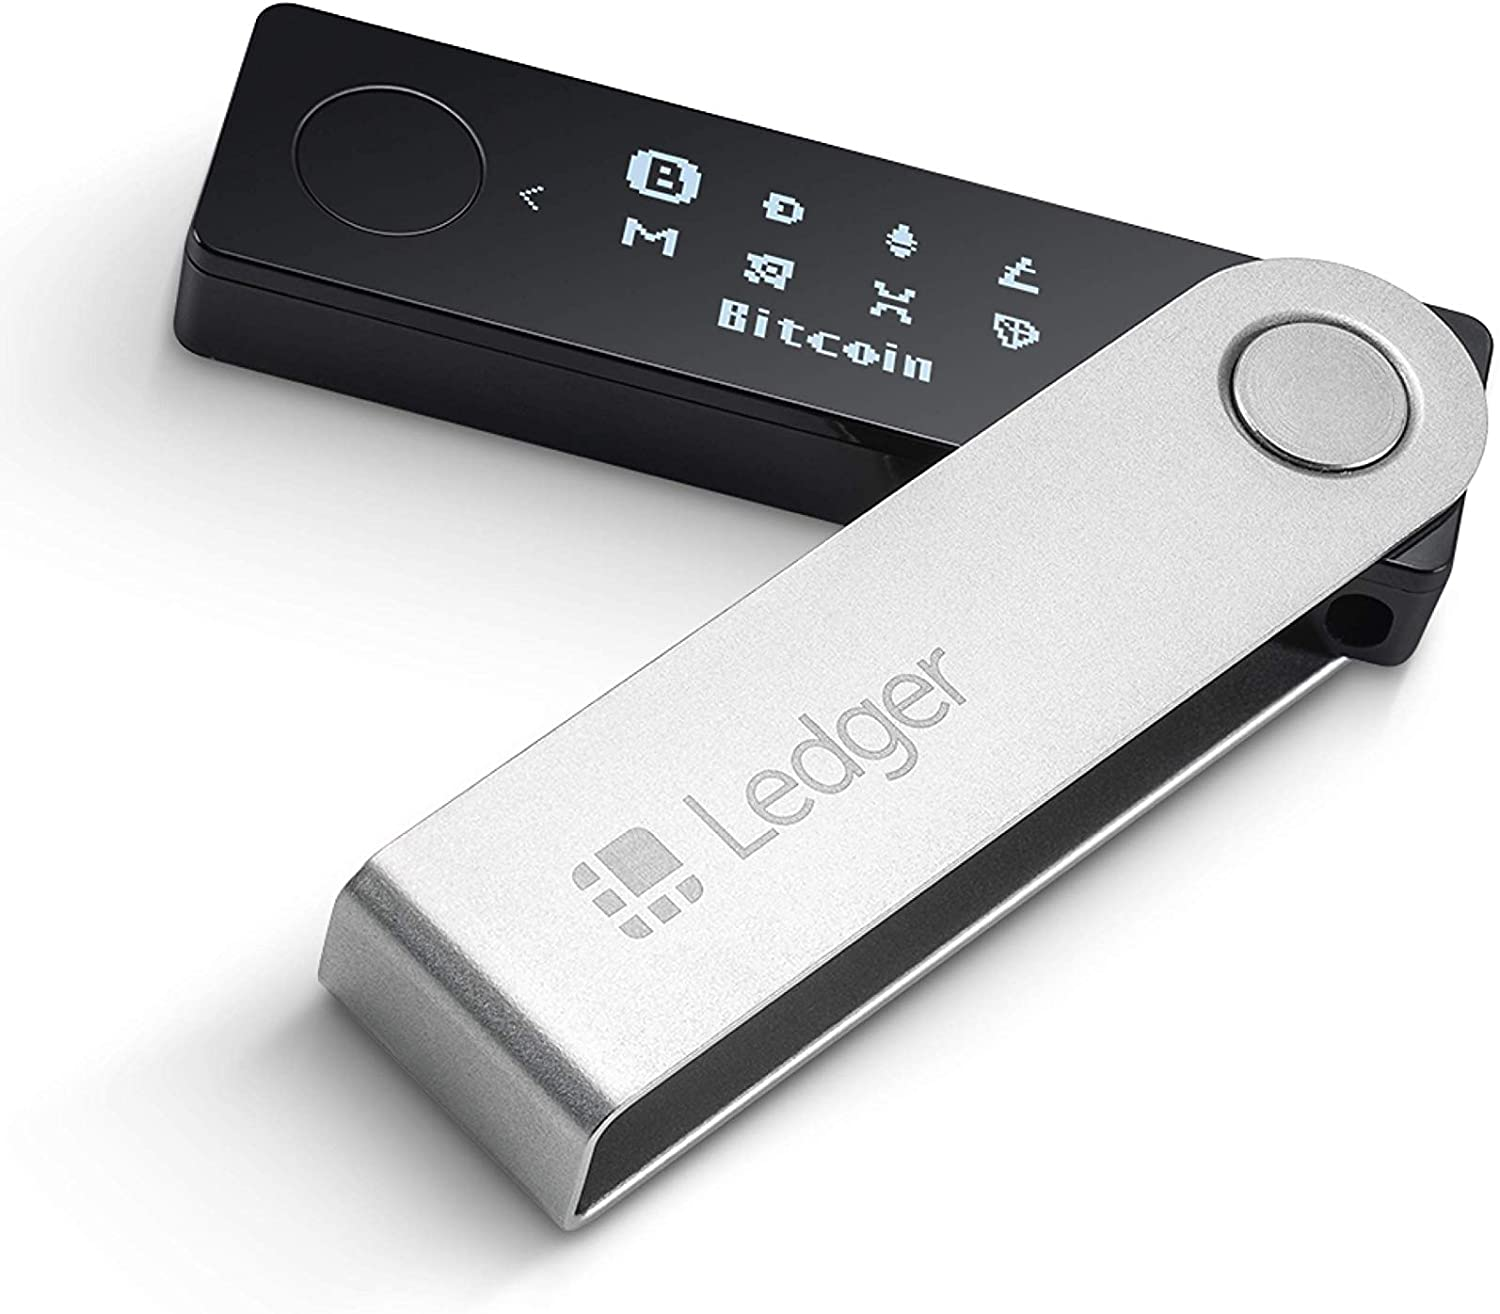
\includegraphics[scale = 0.1]{figures/hardware_wallet.jpg}
%     \caption{An Example of a Hardware Wallet\cite{hard}}
%     \label{fig:hardware_wallet}
% \end{figure}
%
%
% \subsection{HD Wallets}
% For a wallet, we want to generate public and secret key pairs (sk, pk) $\longleftarrow$ $\mathsf{Gen}(1^\kappa)$.
%
% To do this, one approach is to start with a seed that is randomly generated (such as a series of words), then hash the seed with a counter. Note that we cannot use human-generated random words, such as ``I love my dog", because it could be easily stolen.
%
% One commonly used approach is the following. Given a randomly generated \textit{seed}, we can concatenate it with a counter and hash the concatenation to achieve a new secret key. Then, from the secret key, we can generate a public key.
% \begin{align*}
% H(\text{ctr}\|\text{seed})&\longrightarrow \text{new sk} \\
% H(1\|\text{seed}) &\longrightarrow \text{new sk}_0  \\
% H(2\|\text{seed}) &\longrightarrow \text{new sk}_1 \\
% &\cdots
% \end{align*}
%
\section*{Problems}
TBD

\section*{Further Reading}
While it is folklore belief that a cryptocurrency can remain incentive-compatible
when payouts consists only of block rewards and no fees, this belief is actually
false. This was studied in the paper
\emph{On the Instability of Bitcoin Without the Block Reward}~\cite{instability}.

The field of optimizing miner strategies was pioneered by two works,
\emph{Clockwork Finance}~\cite{clockwork} and \emph{FlashBoys 2.0}~\cite{flashboys}.
These gave rise to the concept of \emph{MEV}, or Miner Extractable Value, and
gave rise to a whole industry of \emph{searchers}, \emph{builders}, and \emph{proposers},
allocating different roles to the different portions pertaining to this optimization
problem. The most popular platform in the field currently concerning itself with
such optimizations is \emph{FlashBots}.

The taxonomy of various wallets was studied in
\emph{A Taxonomy of Cryptocurrency Wallets}~\cite{wallet-taxonomy}, where various
types of wallets are described. The security of hardware wallets is analyzed in
\emph{A Formal Treatment of Hardware Wallets}~\cite{hardware-wallets}.

The way keys are generated from seeds depends on the particular blockchain.
The first blockchain to use seeds was Bitcoin. The structure that Bitcoin
uses is complex and is described in technical detail in the standards
BIP32~\cite{bip32}, BIP39~\cite{bip39}, and BIP44~\cite{bip44}.

% TODO: briefly describe the Bahack attack in the main text
% after the backbone chapters

The target recalculation formula given in this chapter is a simplified
version of the real formula. The real formula contains a \emph{clamping
parameter}. Constructing a variable difficulty protocol is not a simple
matter. There are insidious attacks that can appear. One prominent such
attack is due to Bahack~\cite{bahack}. For the detailed analysis of the
security of the variable difficulty protocol, consult the seminal
work \emph{The Bitcoin Backbone Protocol with Chains of Variable
Difficulty}~\cite{varbackbone}.
